% !TeX root = ../../thesis.tex
\chapter{Temperature-Dependent Properties of \ch{CsPbI2Br} Thin Films}\label{ch:ellipsometry}


\begin{itemize}
    \item Correlation between optoelectronic properties/Structural Properties and device performance - association with film annealing
    \item In the previous chapter we showed how we performed in situ GIWAXS to identify the phase transition temperatures and crystallite size 
    \item However GIWAXS is a synchrotron base technique and required access to synchrotron facilities, this can be costly and not easily accessible for many labs
    \item Need for measurements with fast enough acquisition time that can be easily accessible (for example XRD is commonly used, but measuring each angle can take a long time) - give some other examples 
    \item This is how we turned our attention to spectroscopic ellipsometry

\end{itemize}

\section{Temperature-Dependent Spectroscopic Ellipsometry}

\begin{itemize}
    \item Fundamentals of Spectroscopic Ellipsometry
    \item Room Temperature Characterization of Perovskite Thin Films
    \item Temperature-dependent works in literature
\end{itemize}

\subsection{Model Development for Temperature-Dependent Measurements}

\begin{itemize}
    \item 1st Option: Multiple models at different temperature intervals
    \item 2nd Option: Model at the beginning of the experiment, fit in real time
    \item 3rd Option: Dynamic Model based on selected timestamps
\end{itemize}

\begin{figure}[htbp]
    \centering
    % First plot
    \begin{subfigure}[t]{0.95\textwidth} % Adjust width if needed
        \centering
        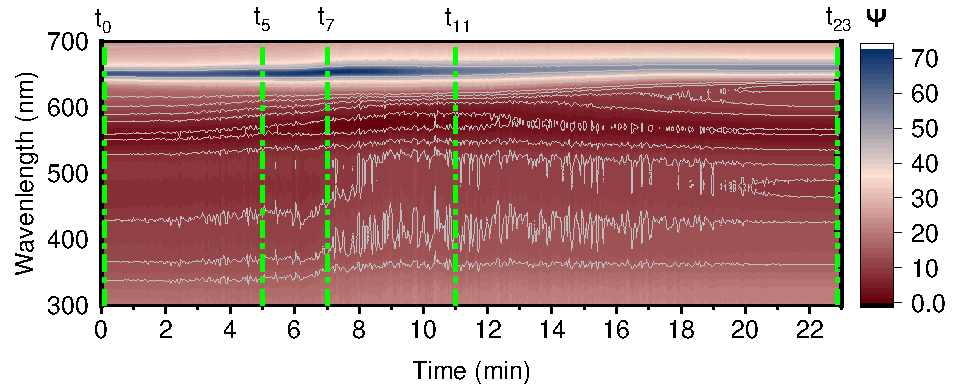
\includegraphics[width=\textwidth]{chapters/ellipsometry/image/Psi_Contour - MRS.pdf} % Replace with your image
        %\caption{Description for subplot (a).}
        %\label{fig:sub-a}
    \end{subfigure}

    \vspace{1em} % Space between the rows

    % Second plot
    \begin{subfigure}[t]{0.95\textwidth} % Adjust width if needed
        \centering
        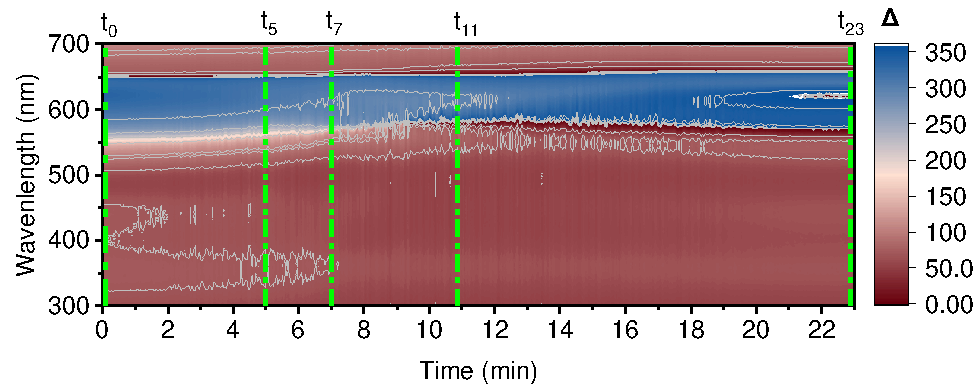
\includegraphics[width=\textwidth]{chapters/ellipsometry/image/Delta_Contour - MRS.pdf} % Replace with your image
        %\caption{Description for subplot (b).}
        %\label{fig:sub-b}
    \end{subfigure}

    % Caption for the whole figure
    \caption{Evolution of raw ellipsometry data as a function of time and temperature for various wavelengths. The data range has been limited to 300 - 700 nm for a clearer visual representation. The green dashed lines indicate the timestamps for which a static model was developed.}
    \label{fig:ellipsometry:raw_psi_delta}
\end{figure}



\begin{figure}
  \centering
  \medskip
  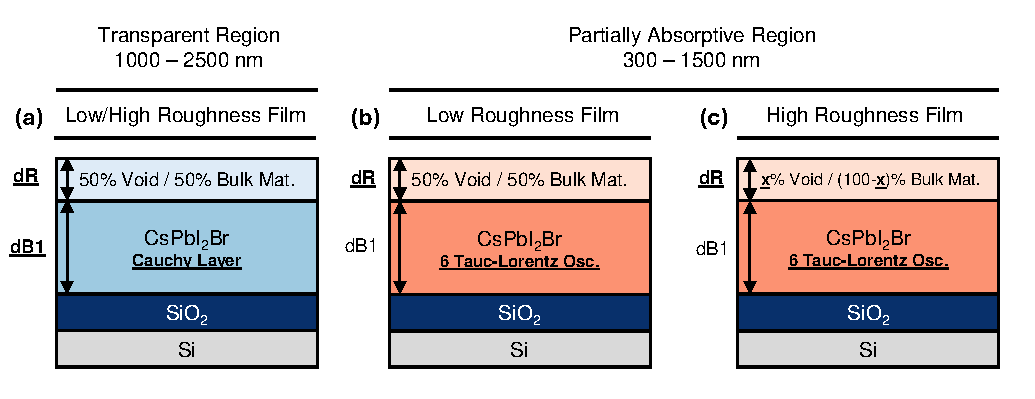
\includegraphics[width=.95\textwidth]{chapters/ellipsometry/image/Model_Approach.pdf}
  \caption{Schematics of the optical models used for static ellipsometry fitting, depending on the transparency and roughness of the perovskite film. The bold and underlined text indicates the fitting parameters. For the models in the partially absorptive region, the bulk perovskite thickness (dB1) is fixed to the value calculated through the transparent region model.}
  \label{fig:ellipsometry:static_models}
\end{figure}


\begin{figure}[htbp]
    \centering
    % First row
    \begin{subfigure}[t]{0.45\textwidth}
        \centering
        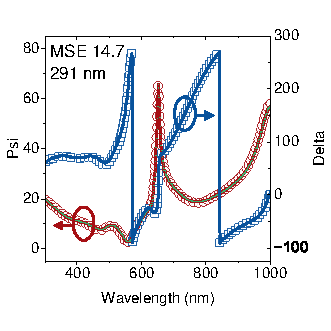
\includegraphics[width=\textwidth]{chapters/ellipsometry/image/t0_plot.pdf} % Replace with your image file
        \caption{As-Deposited State}
        \label{fig:ellipsometry:static_fits:t0}
    \end{subfigure}
    \hfill
    \begin{subfigure}[t]{0.45\textwidth}
        \centering
        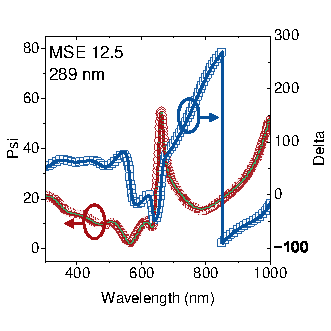
\includegraphics[width=\textwidth]{chapters/ellipsometry/image/t23_fixed_thick_x_void_p.pdf} 
        \label{fig:ellipsometry:static_fits:t23_fixed_thick_x_void}
        % Replace with your image file
        \caption{Annealed State - Model A}
    \end{subfigure}

    %\vspace{1em} % Space between rows

    % Second row
    \begin{subfigure}[t]{0.45\textwidth}
        \centering
        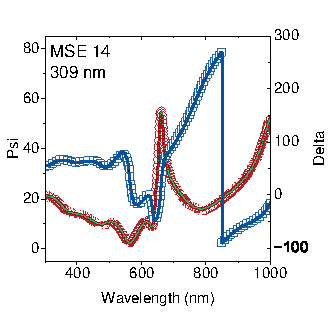
\includegraphics[width=\textwidth]{chapters/ellipsometry/image/t23_fitted_thickness.pdf} % Replace with your image file
        \caption{Annealed State - Model B}
        \label{fig:ellipsometry:static_fits:t23_fitted_thick}
    \end{subfigure}
    \hfill
    \begin{subfigure}[t]{0.45\textwidth}
        \centering
        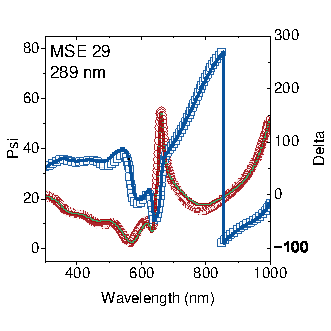
\includegraphics[width=\textwidth]{chapters/ellipsometry/image/t23_fixed_thickness_50_v.pdf} % Replace with your image file
        \caption{Annealed State - Model C}
        \label{fig:ellipsometry:static_fits:t23_fixed_thick_50_void}
    \end{subfigure}
    \caption{Comparison between SE experimental data (open symbols) and fitted results (solid lines).}
    \label{fig:ellipsometry:static_fits}
\end{figure}


\begin{figure}[htbp]
    \centering
    % First row
    \begin{subfigure}[t]{0.4\textwidth}
        \centering
        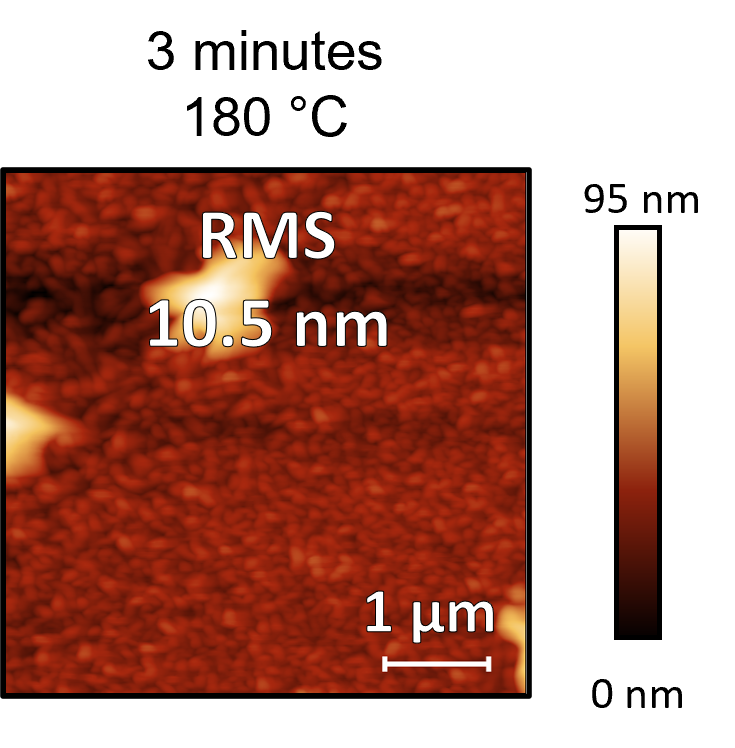
\includegraphics[width=\textwidth]{chapters/ellipsometry/image/180C_3min.png} % Replace with your image file
        \caption*{(a)}
    \end{subfigure}
    \hfill
    \begin{subfigure}[t]{0.4\textwidth}
        \centering
        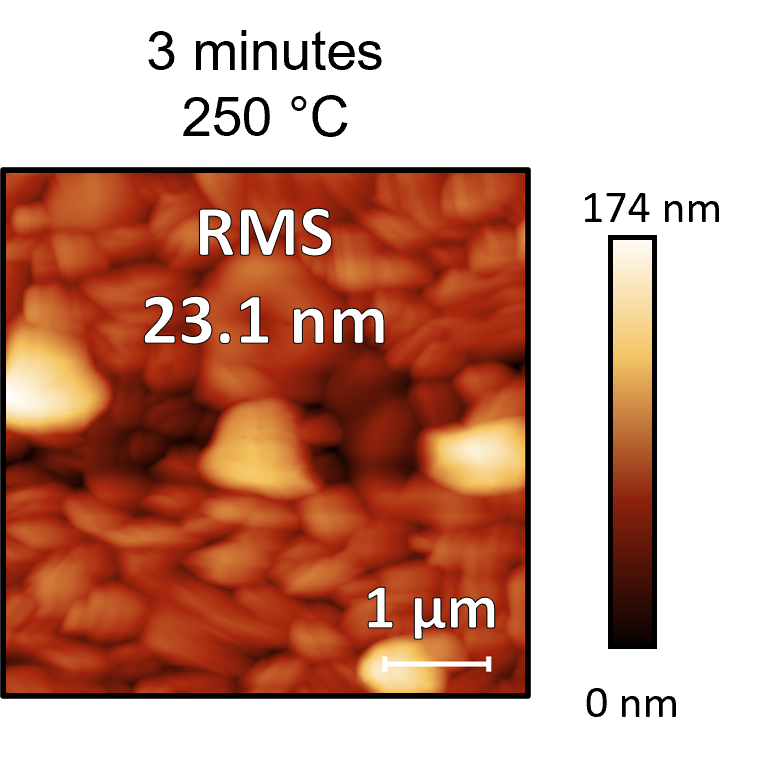
\includegraphics[width=\textwidth]{chapters/ellipsometry/image/250C_3min.png} % Replace with your image file
        \caption*{(b)}
    \end{subfigure}

    \vspace{1em} % Space between rows

    % Second row
    \begin{subfigure}[t]{0.4\textwidth}
        \centering
        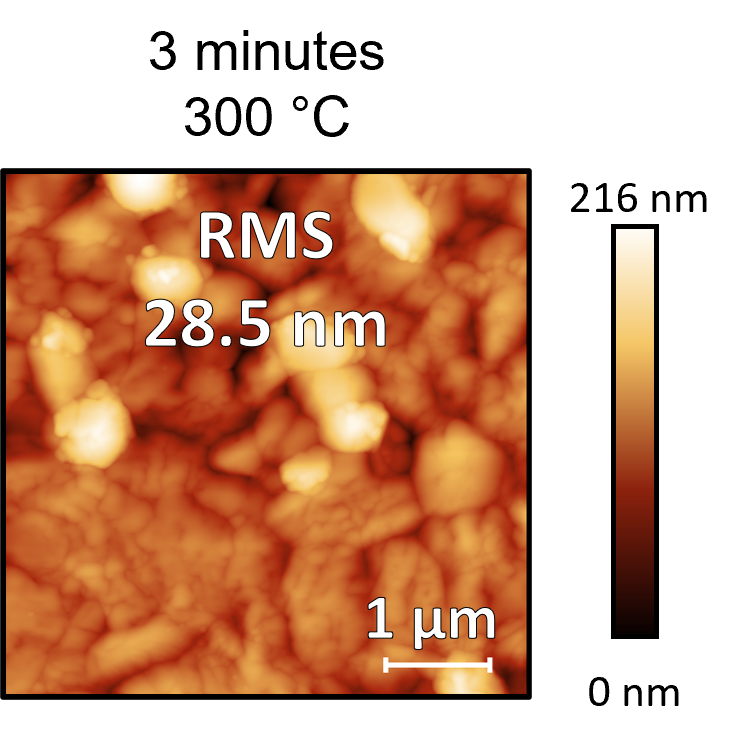
\includegraphics[width=\textwidth]{chapters/ellipsometry/image/300C_3min.png} % Replace with your image file
        \caption*{(c)}
    \end{subfigure}
    \hfill
    \begin{subfigure}[t]{0.4\textwidth}
        \centering
        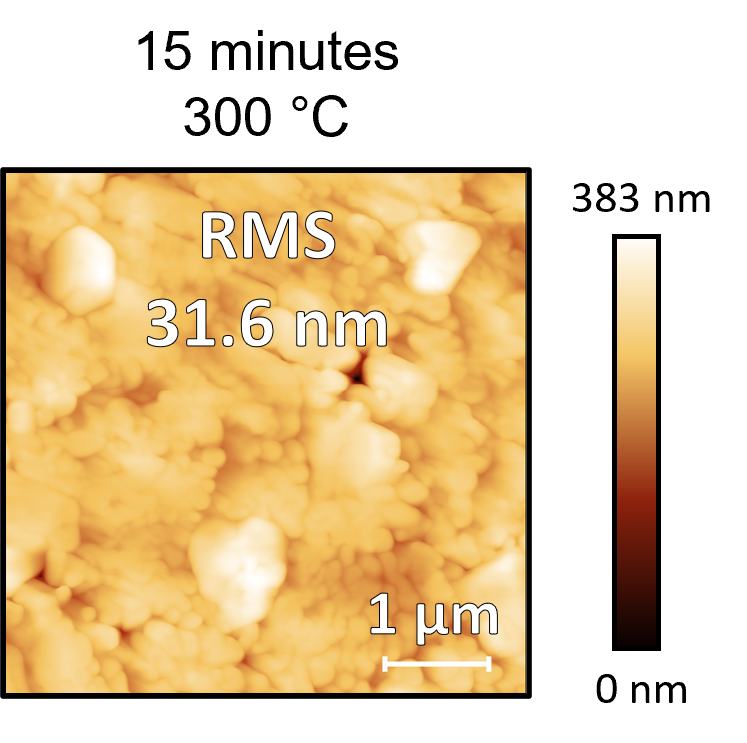
\includegraphics[width=\textwidth]{chapters/ellipsometry/image/300C_15min.png} % Replace with your image file
        \caption*{(d)}
    \end{subfigure}
    \caption{AFM image of the \ch{CsPbI2Br} sample annealed (a) for 3 minutes at 180\degree C, (b) for 3 minutes at 250\degree C, (c) for 3 minutes at 300\degree C, and (d) for 15 minutes at 300\degree C.}
\end{figure}





\begin{figure}
  \centering
  \medskip
  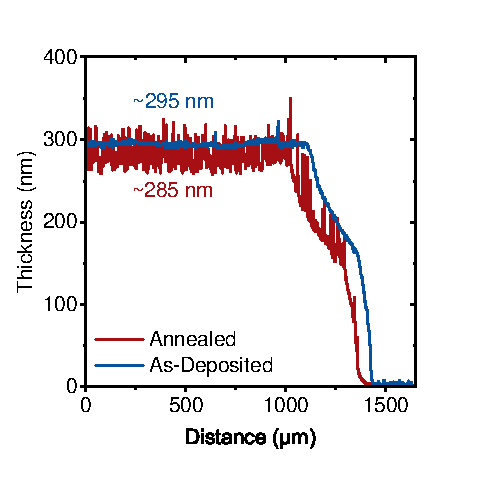
\includegraphics[width=.5\textwidth]{chapters/ellipsometry/image/Dektak.pdf}
  \caption{Profilometry results for the As-Deposited and Annealed state.}
  \label{fig:ellipsometry:profilometry}
\end{figure}



\begin{figure}
  \centering
  \medskip
  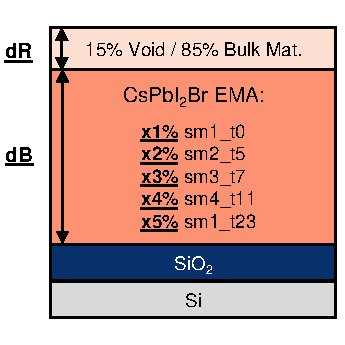
\includegraphics[width=.45\textwidth]{chapters/ellipsometry/image/Dynamic_Model.pdf}
  \caption{Schematic of the optical model used for the dynamic ellipsometry fitting. The bulk layer consists of the five static models shown in \ref{fig:ellipsometry:raw_psi_delta}. The parameters fo these models are fixed, but the percentage of their volume fraction is fitted. The roughness layer consists of 15\% voids.}
  \label{fig:ellipsometry:dynamic_model}
\end{figure}



\section{In situ annealing annealing effect on Morphology}

\begin{figure}
  \centering
  \medskip
  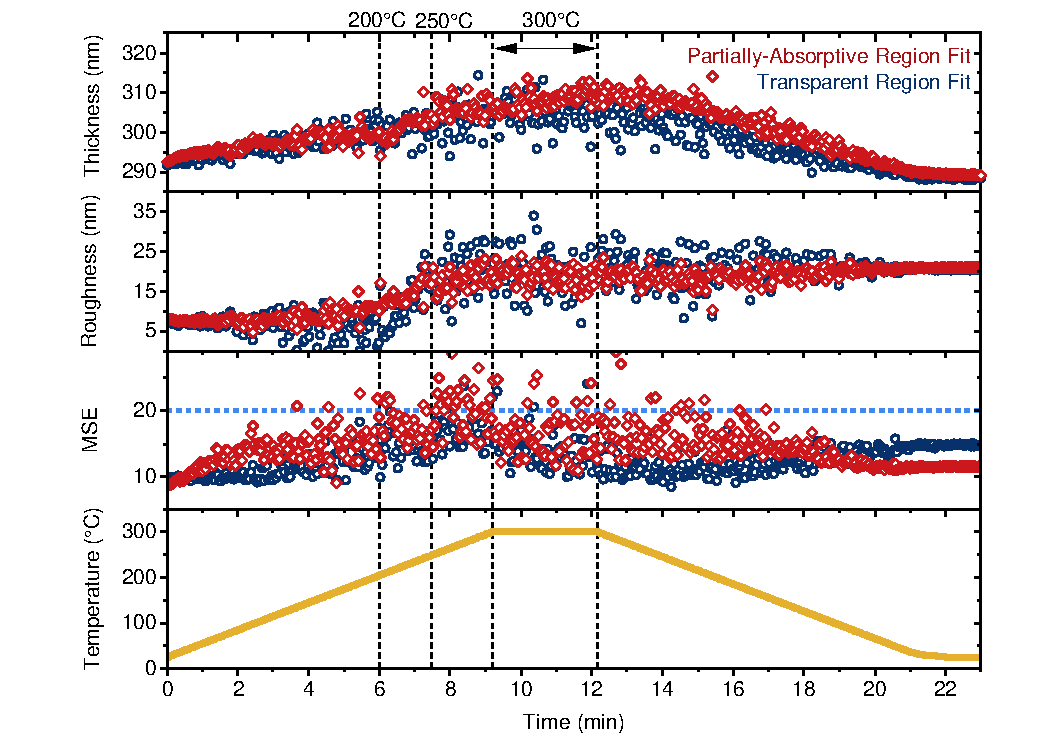
\includegraphics[width=.99\textwidth]{chapters/ellipsometry/image/Roughness_Thickness.pdf}
  \caption{Evolution of the \ch{CsPbI2Br} film's thickness and roughness, as well as the fit's MSE, as a function ot time and temperature according to our dynamic SE model.}
  \label{fig:ellipsometry:roughness_thickness}
\end{figure}


\subsection{Thickness}
\subsection{Roughness}
\section{In situ annealing annealing effect on Optical Constants}

\begin{figure}
  \centering
  \medskip
  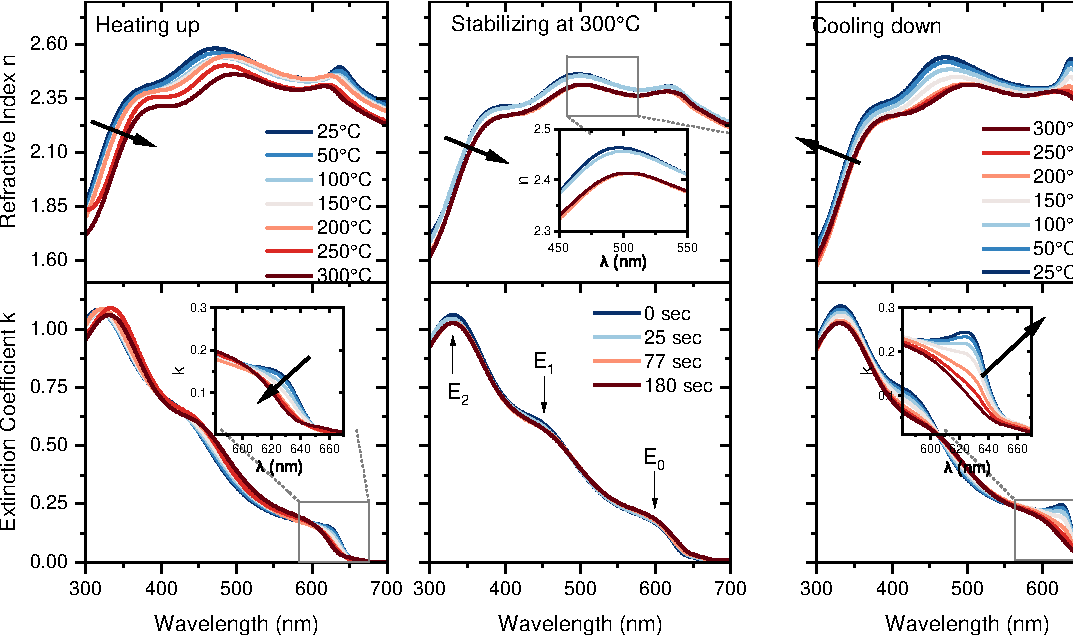
\includegraphics[width=.99\textwidth]{chapters/ellipsometry/image/Optical_constants.pdf}
  \caption{Evolution of the \ch{CsPbI2Br} film's refractive index (n) and extinction coefficient (k).}
  \label{fig:ellipsometry:optical_constants}
\end{figure}


\subsection{Thermo-Optic Coefficient}

\begin{figure}[htbp]
    \centering
    \begin{subfigure}{0.32\textwidth}
        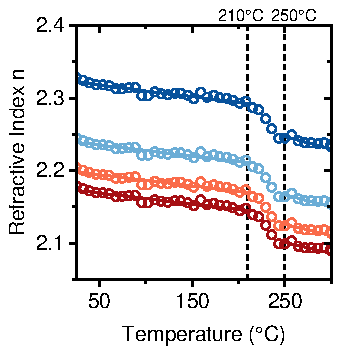
\includegraphics[width=\textwidth]{chapters/ellipsometry/image/Thermo-optic_Coefficient_heating.pdf}
        \caption{}
        \label{fig:ellipsometry:thermooptic_heating}
    \end{subfigure}
    \hfill
    \begin{subfigure}{0.32\textwidth}
        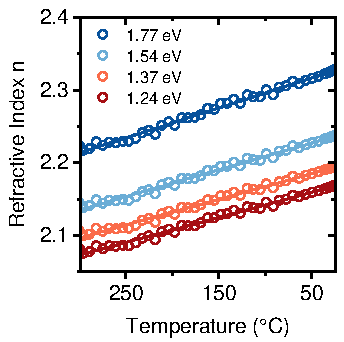
\includegraphics[width=\textwidth]{chapters/ellipsometry/image/Thermo-optic_Coefficient_cooling.pdf}
        \caption{}
        \label{fig:ellipsometry:thermooptic_cooling}
    \end{subfigure}
    \hfill
    \begin{subfigure}{0.3\textwidth}
        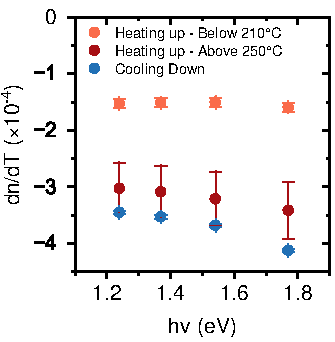
\includegraphics[width=\textwidth]{chapters/ellipsometry/image/Thermo-optic_Coefficient_energy.pdf}
        \caption{}
        \label{fig:ellipsometry:thermooptic_energy}
    \end{subfigure}
    \caption{A 1x3 figure layout.}
    \label{fig:ellipsometry:thermooptic}
\end{figure}



\subsection{Urbach Energy}

\begin{figure}[htbp]
    \centering
    \begin{subfigure}{0.32\textwidth}
        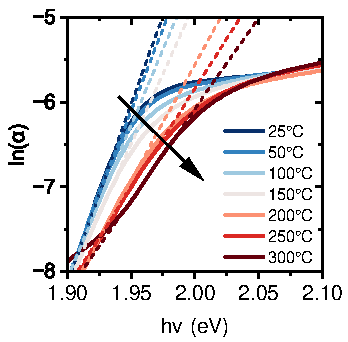
\includegraphics[width=\textwidth]{chapters/ellipsometry/image/Urbach_heating.pdf}
        \caption{}
        \label{fig:ellipsometry:urbach_heating}
    \end{subfigure}
    \hfill
    \begin{subfigure}{0.32\textwidth}
        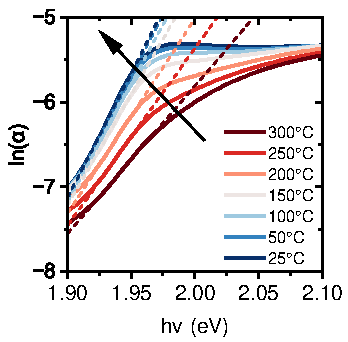
\includegraphics[width=\textwidth]{chapters/ellipsometry/image/Urbach_cooling.pdf}
        \caption{}
        \label{fig:ellipsometry:urbach_cooling}
    \end{subfigure}
    \hfill
    \begin{subfigure}{0.3\textwidth}
        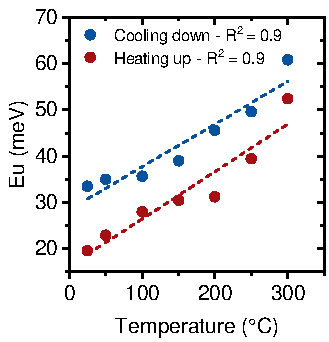
\includegraphics[width=\textwidth]{chapters/ellipsometry/image/Urbach_temp.pdf}
        \caption{}
        \label{fig:ellipsometry:urbach_temp}
    \end{subfigure}
    \caption{A 1x3 figure layout.}
    \label{fig:ellipsometry:urbach}
\end{figure}


\subsection{Critical Point Analysis}

\begin{figure}[htbp]
    \centering
    \begin{subfigure}{0.34\textwidth}
        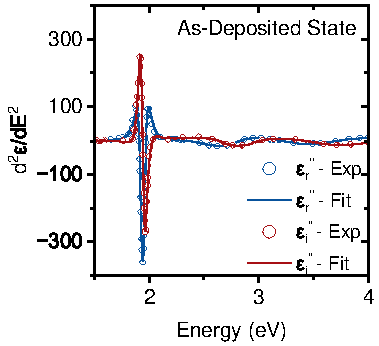
\includegraphics[width=\textwidth]{chapters/ellipsometry/image/Deriv_As_Dep.pdf}
        \caption{}
        \label{fig:ellipsometry:deriv:As_dep}
    \end{subfigure}
    \hfill
    \begin{subfigure}{0.31\textwidth}
        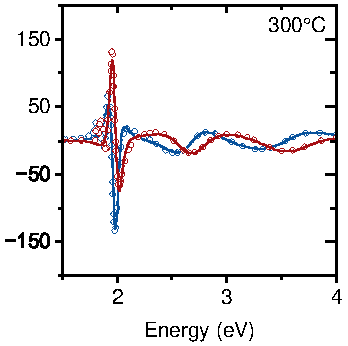
\includegraphics[width=\textwidth]{chapters/ellipsometry/image/Deriv_300C.pdf}
        \caption{}
        \label{fig:ellipsometry:deriv:300}
    \end{subfigure}
    \hfill
    \begin{subfigure}{0.31\textwidth}
        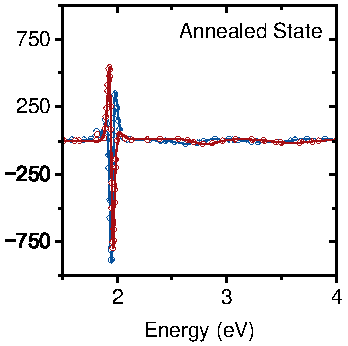
\includegraphics[width=\textwidth]{chapters/ellipsometry/image/Deriv_Anneal.pdf}
        \caption{}
        \label{fig:ellipsometry:deriv:anneal}
    \end{subfigure}
    \caption{A 1x3 figure layout.}
    \label{fig:ellipsometry:deriv}
\end{figure}

\begin{figure}[htbp]
    \centering
    \begin{subfigure}{0.34\textwidth}
        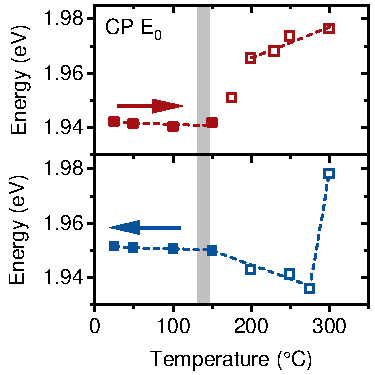
\includegraphics[width=\textwidth]{chapters/ellipsometry/image/CP0.pdf}
        \caption{}
        \label{fig:ellipsometry:CP0}
    \end{subfigure}
    \hfill
    \begin{subfigure}{0.31\textwidth}
        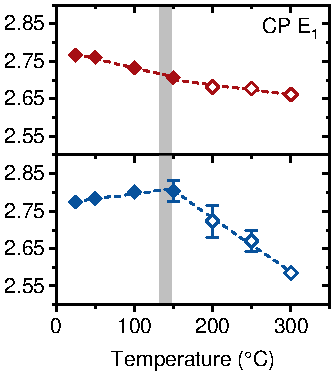
\includegraphics[width=\textwidth]{chapters/ellipsometry/image/CP1.pdf}
        \caption{}
        \label{fig:ellipsometry:CP1}
    \end{subfigure}
    \hfill
    \begin{subfigure}{0.31\textwidth}
        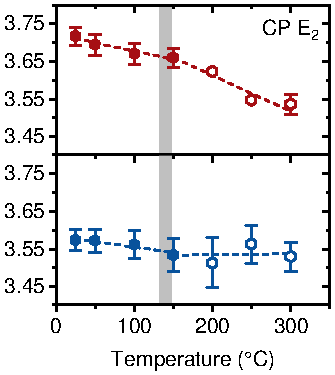
\includegraphics[width=\textwidth]{chapters/ellipsometry/image/CP3}
        \caption{}
        \label{fig:ellipsometry:deriv:CP2}
    \end{subfigure}
    \caption{A 1x3 figure layout.}
    \label{fig:ellipsometry:CP_all}
\end{figure}



\section{Conclusions}


%%%%%%%%%%%%%%%%%%%%%%%%%%%%%%%%%%%%%%%%%%%%%%%%%%
% Keep the following \cleardoublepage at the end of this file, 
% otherwise \includeonly includes empty pages.
\cleardoublepage

